\documentclass{standalone}
\usepackage{tikz}
\usetikzlibrary{patterns, positioning}


\begin{document}
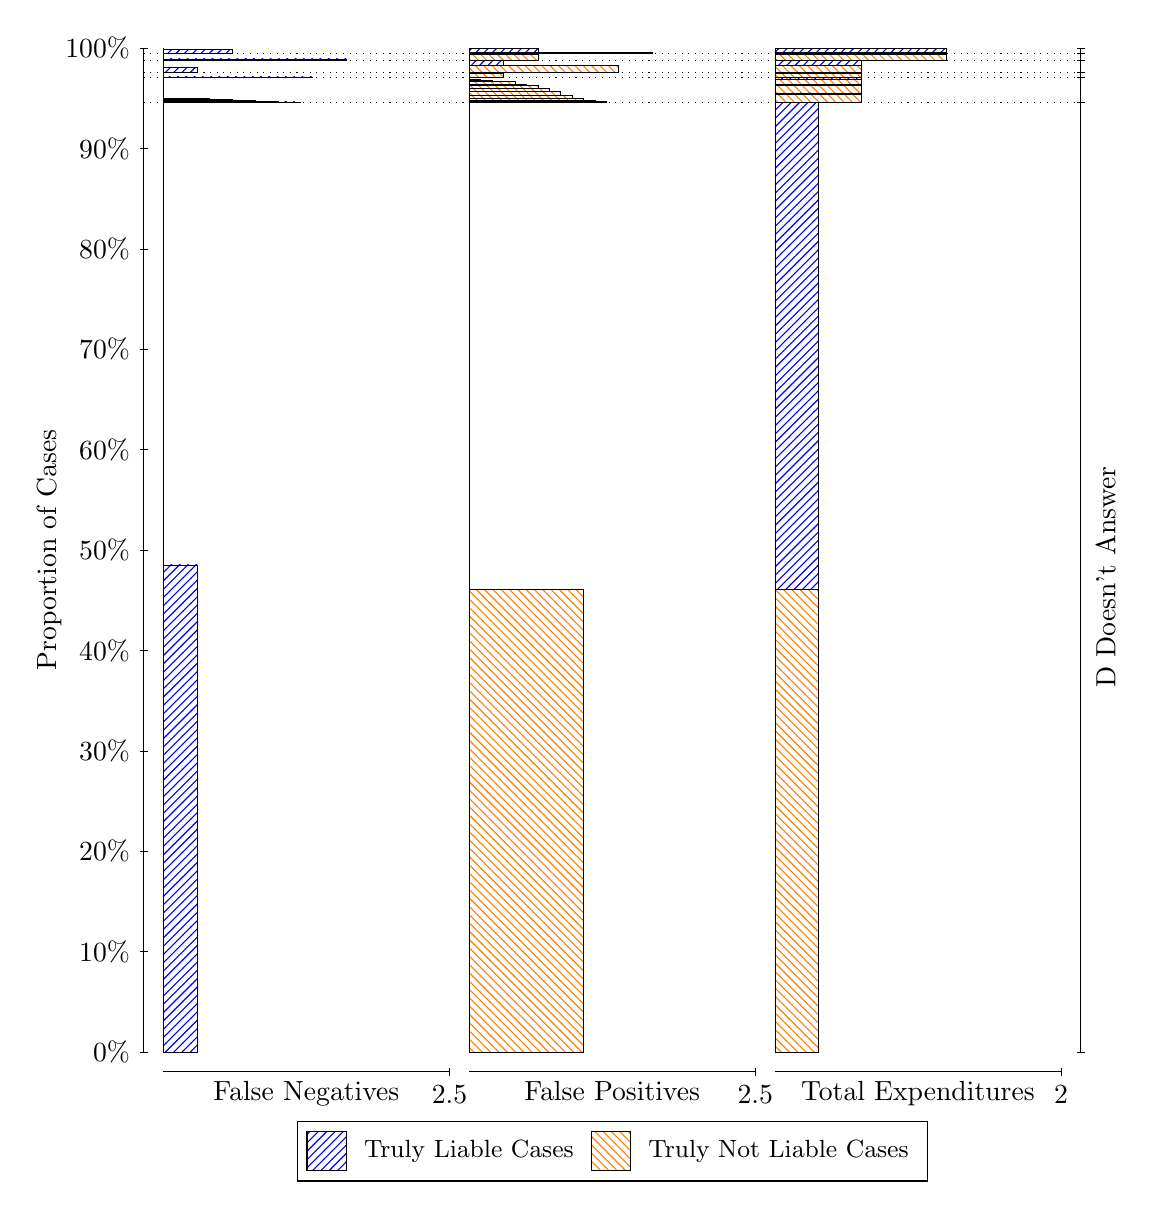
\begin{tikzpicture}
\draw[black, very thin] (1.5,1.75) -- (1.5,14.5);
\node[rotate=90, text=black, anchor=center] at (0.3, 8.125) {Proportion of Cases};
\draw[black, very thin] (1.45,1.75) -- (1.55,1.75);
\node[text=black, anchor=east] at (1.45, 1.75) {0\%};
\draw[black, very thin] (1.45,3.025) -- (1.55,3.025);
\node[text=black, anchor=east] at (1.45, 3.025) {10\%};
\draw[black, very thin] (1.45,4.3) -- (1.55,4.3);
\node[text=black, anchor=east] at (1.45, 4.3) {20\%};
\draw[black, very thin] (1.45,5.575) -- (1.55,5.575);
\node[text=black, anchor=east] at (1.45, 5.575) {30\%};
\draw[black, very thin] (1.45,6.85) -- (1.55,6.85);
\node[text=black, anchor=east] at (1.45, 6.85) {40\%};
\draw[black, very thin] (1.45,8.125) -- (1.55,8.125);
\node[text=black, anchor=east] at (1.45, 8.125) {50\%};
\draw[black, very thin] (1.45,9.4) -- (1.55,9.4);
\node[text=black, anchor=east] at (1.45, 9.4) {60\%};
\draw[black, very thin] (1.45,10.675) -- (1.55,10.675);
\node[text=black, anchor=east] at (1.45, 10.675) {70\%};
\draw[black, very thin] (1.45,11.95) -- (1.55,11.95);
\node[text=black, anchor=east] at (1.45, 11.95) {80\%};
\draw[black, very thin] (1.45,13.225) -- (1.55,13.225);
\node[text=black, anchor=east] at (1.45, 13.225) {90\%};
\draw[black, very thin] (1.45,14.5) -- (1.55,14.5);
\node[text=black, anchor=east] at (1.45, 14.5) {100\%};

\draw[black, very thin] (13.4,1.75) -- (13.4,14.5);
\draw[black, very thin] (13.35,1.75) -- (13.45,1.75);
\node[anchor=west] at (13.35, 1.75) {};
\draw[black, very thin] (13.35,13.812) -- (13.45,13.812);
\node[anchor=west] at (13.35, 13.812) {};
\draw[black, very thin] (13.35,14.129) -- (13.45,14.129);
\node[anchor=west] at (13.35, 14.129) {};
\draw[black, very thin] (13.35,14.19) -- (13.45,14.19);
\node[anchor=west] at (13.35, 14.19) {};
\draw[black, very thin] (13.35,14.344) -- (13.45,14.344);
\node[anchor=west] at (13.35, 14.344) {};
\draw[black, very thin] (13.35,14.434) -- (13.45,14.434);
\node[anchor=west] at (13.35, 14.434) {};
\draw[black, very thin] (13.35,14.5) -- (13.45,14.5);
\node[anchor=west] at (13.35, 14.5) {};

\draw[black, very thin, pattern color=blue, pattern=north east lines] (1.75,1.75) rectangle (2.186,7.9361);
\draw[black, very thin, pattern color=orange, pattern=north west lines] (1.75,7.9361) rectangle (1.75,13.812);
\draw[black, very thin, pattern color=blue, pattern=north east lines] (1.75,13.812) rectangle (3.494,13.815);
\draw[black, very thin, pattern color=blue, pattern=north east lines] (1.75,13.815) rectangle (3.3487,13.817);
\draw[black, very thin, pattern color=blue, pattern=north east lines] (1.75,13.817) rectangle (3.2033,13.821);
\draw[black, very thin, pattern color=blue, pattern=north east lines] (1.75,13.821) rectangle (3.058,13.822);
\draw[black, very thin, pattern color=blue, pattern=north east lines] (1.75,13.822) rectangle (3.058,13.826);
\draw[black, very thin, pattern color=blue, pattern=north east lines] (1.75,13.826) rectangle (2.9127,13.832);
\draw[black, very thin, pattern color=blue, pattern=north east lines] (1.75,13.832) rectangle (2.7673,13.836);
\draw[black, very thin, pattern color=blue, pattern=north east lines] (1.75,13.836) rectangle (2.622,13.843);
\draw[black, very thin, pattern color=blue, pattern=north east lines] (1.75,13.843) rectangle (2.4767,13.849);
\draw[black, very thin, pattern color=blue, pattern=north east lines] (1.75,13.849) rectangle (2.3313,13.863);
\draw[black, very thin, pattern color=orange, pattern=north west lines] (1.75,13.863) rectangle (1.75,14.129);
\draw[black, very thin, pattern color=blue, pattern=north east lines] (1.75,14.129) rectangle (3.6393,14.134);
\draw[black, very thin, pattern color=orange, pattern=north west lines] (1.75,14.134) rectangle (1.75,14.19);
\draw[black, very thin, pattern color=blue, pattern=north east lines] (1.75,14.19) rectangle (2.186,14.255);
\draw[black, very thin, pattern color=orange, pattern=north west lines] (1.75,14.255) rectangle (1.75,14.344);
\draw[black, very thin, pattern color=blue, pattern=north east lines] (1.75,14.344) rectangle (4.0753,14.361);
\draw[black, very thin, pattern color=orange, pattern=north west lines] (1.75,14.361) rectangle (1.75,14.434);
\draw[black, very thin, pattern color=blue, pattern=north east lines] (1.75,14.434) rectangle (2.622,14.485);
\draw[black, very thin, pattern color=orange, pattern=north west lines] (1.75,14.485) rectangle (1.75,14.5);
\draw[black, very thin, pattern color=orange, pattern=north west lines] (5.6333,1.75) rectangle (7.0867,7.6256);
\draw[black, very thin, pattern color=blue, pattern=north east lines] (5.6333,7.6256) rectangle (5.6333,13.812);
\draw[black, very thin, pattern color=orange, pattern=north west lines] (5.6333,13.812) rectangle (7.3773,13.818);
\draw[black, very thin, pattern color=orange, pattern=north west lines] (5.6333,13.818) rectangle (7.232,13.832);
\draw[black, very thin, pattern color=orange, pattern=north west lines] (5.6333,13.832) rectangle (7.0867,13.862);
\draw[black, very thin, pattern color=orange, pattern=north west lines] (5.6333,13.862) rectangle (6.9413,13.896);
\draw[black, very thin, pattern color=orange, pattern=north west lines] (5.6333,13.896) rectangle (6.796,13.951);
\draw[black, very thin, pattern color=orange, pattern=north west lines] (5.6333,13.951) rectangle (6.6507,13.992);
\draw[black, very thin, pattern color=orange, pattern=north west lines] (5.6333,13.992) rectangle (6.5053,14.03);
\draw[black, very thin, pattern color=orange, pattern=north west lines] (5.6333,14.03) rectangle (6.36,14.043);
\draw[black, very thin, pattern color=orange, pattern=north west lines] (5.6333,14.043) rectangle (6.2147,14.077);
\draw[black, very thin, pattern color=blue, pattern=north east lines] (5.6333,14.077) rectangle (5.924,14.092);
\draw[black, very thin, pattern color=blue, pattern=north east lines] (5.6333,14.092) rectangle (5.7787,14.097);
\draw[black, very thin, pattern color=blue, pattern=north east lines] (5.6333,14.097) rectangle (5.6333,14.129);
\draw[black, very thin, pattern color=orange, pattern=north west lines] (5.6333,14.129) rectangle (6.0693,14.185);
\draw[black, very thin, pattern color=blue, pattern=north east lines] (5.6333,14.185) rectangle (5.6333,14.19);
\draw[black, very thin, pattern color=orange, pattern=north west lines] (5.6333,14.19) rectangle (7.5227,14.279);
\draw[black, very thin, pattern color=blue, pattern=north east lines] (5.6333,14.279) rectangle (6.0693,14.344);
\draw[black, very thin, pattern color=orange, pattern=north west lines] (5.6333,14.344) rectangle (6.5053,14.417);
\draw[black, very thin, pattern color=blue, pattern=north east lines] (5.6333,14.417) rectangle (5.6333,14.434);
\draw[black, very thin, pattern color=orange, pattern=north west lines] (5.6333,14.434) rectangle (7.9587,14.449);
\draw[black, very thin, pattern color=blue, pattern=north east lines] (5.6333,14.449) rectangle (6.5053,14.5);
\draw[black, very thin, pattern color=orange, pattern=north west lines] (9.5167,1.75) rectangle (10.062,7.6256);
\draw[black, very thin, pattern color=blue, pattern=north east lines] (9.5167,7.6256) rectangle (10.062,13.812);
\draw[black, very thin, pattern color=orange, pattern=north west lines] (9.5167,13.812) rectangle (10.607,13.91);
\draw[black, very thin, pattern color=blue, pattern=north east lines] (9.5167,13.91) rectangle (10.607,13.929);
\draw[black, very thin, pattern color=orange, pattern=north west lines] (9.5167,13.929) rectangle (10.607,14.028);
\draw[black, very thin, pattern color=blue, pattern=north east lines] (9.5167,14.028) rectangle (10.607,14.038);
\draw[black, very thin, pattern color=orange, pattern=north west lines] (9.5167,14.038) rectangle (10.607,14.107);
\draw[black, very thin, pattern color=blue, pattern=north east lines] (9.5167,14.107) rectangle (10.607,14.129);
\draw[black, very thin, pattern color=orange, pattern=north west lines] (9.5167,14.129) rectangle (10.607,14.185);
\draw[black, very thin, pattern color=blue, pattern=north east lines] (9.5167,14.185) rectangle (10.607,14.19);
\draw[black, very thin, pattern color=orange, pattern=north west lines] (9.5167,14.19) rectangle (10.607,14.279);
\draw[black, very thin, pattern color=blue, pattern=north east lines] (9.5167,14.279) rectangle (10.607,14.344);
\draw[black, very thin, pattern color=orange, pattern=north west lines] (9.5167,14.344) rectangle (11.697,14.417);
\draw[black, very thin, pattern color=blue, pattern=north east lines] (9.5167,14.417) rectangle (11.697,14.434);
\draw[black, very thin, pattern color=orange, pattern=north west lines] (9.5167,14.434) rectangle (11.697,14.449);
\draw[black, very thin, pattern color=blue, pattern=north east lines] (9.5167,14.449) rectangle (11.697,14.5);
\draw[black, dotted] (1.5,13.812) -- (13.4,13.812);
\draw[black, dotted] (1.5,14.129) -- (13.4,14.129);
\draw[black, dotted] (1.5,14.19) -- (13.4,14.19);
\draw[black, dotted] (1.5,14.344) -- (13.4,14.344);
\draw[black, dotted] (1.5,14.434) -- (13.4,14.434);
\draw[black, very thin] (1.75,1.5) -- (5.3833,1.5);
\node[text=black, anchor=north] at (3.5667, 1.5) {False Negatives};
\draw[black, very thin] (5.3833,1.45) -- (5.3833,1.55);
\node[text=black, anchor=north] at (5.3833, 1.45) {2.5};

\draw[black, very thin] (5.6333,1.5) -- (9.2667,1.5);
\node[text=black, anchor=north] at (7.45, 1.5) {False Positives};
\draw[black, very thin] (9.2667,1.45) -- (9.2667,1.55);
\node[text=black, anchor=north] at (9.2667, 1.45) {2.5};

\draw[black, very thin] (9.5167,1.5) -- (13.15,1.5);
\node[text=black, anchor=north] at (11.333, 1.5) {Total Expenditures};
\draw[black, very thin] (13.15,1.45) -- (13.15,1.55);
\node[text=black, anchor=north] at (13.15, 1.45) {2};

\node[text=black, centered, rotate=90] at (13.72, 7.7809) {D Doesn't Answer};






\draw (7.449999999999999,1.5) node[draw=none] (baseCoordinate) {};
\begin{scope}[align=center]
        \matrix[scale=0.5, draw=black, below=0.5cm of baseCoordinate, nodes={draw}, column sep=0.1cm]{
            \node[rectangle, draw, minimum width=0.5cm, minimum height=0.5cm, pattern color=blue, pattern=north east lines] {}; &
            \node[draw=none, font=\small, text=black] (B) {Truly Liable Cases}; &
            \node[rectangle, draw, minimum width=0.5cm, minimum height=0.5cm, pattern color=orange, pattern=north west lines] {}; &
            \node[draw=none, font=\small, text=black] (B) {Truly Not Liable Cases}; \\
            };
\end{scope}

\end{tikzpicture}
\end{document}